\documentclass{article}\usepackage[]{graphicx}\usepackage[]{color}
% maxwidth is the original width if it is less than linewidth
% otherwise use linewidth (to make sure the graphics do not exceed the margin)
\makeatletter
\def\maxwidth{ %
  \ifdim\Gin@nat@width>\linewidth
    \linewidth
  \else
    \Gin@nat@width
  \fi
}
\makeatother

\definecolor{fgcolor}{rgb}{0.345, 0.345, 0.345}
\newcommand{\hlnum}[1]{\textcolor[rgb]{0.686,0.059,0.569}{#1}}%
\newcommand{\hlstr}[1]{\textcolor[rgb]{0.192,0.494,0.8}{#1}}%
\newcommand{\hlcom}[1]{\textcolor[rgb]{0.678,0.584,0.686}{\textit{#1}}}%
\newcommand{\hlopt}[1]{\textcolor[rgb]{0,0,0}{#1}}%
\newcommand{\hlstd}[1]{\textcolor[rgb]{0.345,0.345,0.345}{#1}}%
\newcommand{\hlkwa}[1]{\textcolor[rgb]{0.161,0.373,0.58}{\textbf{#1}}}%
\newcommand{\hlkwb}[1]{\textcolor[rgb]{0.69,0.353,0.396}{#1}}%
\newcommand{\hlkwc}[1]{\textcolor[rgb]{0.333,0.667,0.333}{#1}}%
\newcommand{\hlkwd}[1]{\textcolor[rgb]{0.737,0.353,0.396}{\textbf{#1}}}%
\let\hlipl\hlkwb

\usepackage{framed}
\makeatletter
\newenvironment{kframe}{%
 \def\at@end@of@kframe{}%
 \ifinner\ifhmode%
  \def\at@end@of@kframe{\end{minipage}}%
  \begin{minipage}{\columnwidth}%
 \fi\fi%
 \def\FrameCommand##1{\hskip\@totalleftmargin \hskip-\fboxsep
 \colorbox{shadecolor}{##1}\hskip-\fboxsep
     % There is no \\@totalrightmargin, so:
     \hskip-\linewidth \hskip-\@totalleftmargin \hskip\columnwidth}%
 \MakeFramed {\advance\hsize-\width
   \@totalleftmargin\z@ \linewidth\hsize
   \@setminipage}}%
 {\par\unskip\endMakeFramed%
 \at@end@of@kframe}
\makeatother

\definecolor{shadecolor}{rgb}{.97, .97, .97}
\definecolor{messagecolor}{rgb}{0, 0, 0}
\definecolor{warningcolor}{rgb}{1, 0, 1}
\definecolor{errorcolor}{rgb}{1, 0, 0}
\newenvironment{knitrout}{}{} % an empty environment to be redefined in TeX

\usepackage{alltt}
\PassOptionsToPackage{unicode}{hyperref}
\PassOptionsToPackage{naturalnames}{hyperref}
\usepackage{fullpage}
\usepackage[T2A]{fontenc}
\usepackage[utf8]{inputenc}
\usepackage[russian]{babel}
\usepackage{mathrsfs}
\usepackage{amsfonts}
\usepackage{amsmath }
\IfFileExists{upquote.sty}{\usepackage{upquote}}{}
\begin{document}
\title{Отчет по домашнему заданию}
\pretitle{\vspace{\droptitle}\centering\huge}
\posttitle{\par}
\author{Фахртдинов Т. А.}


\maketitle
Шестая задача. Проверка гипотез однородности для независимых
выборок.

Вариант 3.

\begin{knitrout}
\definecolor{shadecolor}{rgb}{0.969, 0.969, 0.969}\color{fgcolor}\begin{kframe}
\begin{alltt}
\hlstd{TX} \hlkwb{<-} \hlkwd{c}\hlstd{(}\hlnum{27.6}\hlstd{,} \hlnum{20.9}\hlstd{,} \hlnum{55.6}\hlstd{,} \hlnum{69}\hlstd{,} \hlnum{23}\hlstd{,} \hlnum{19.5}\hlstd{,} \hlnum{8.9}\hlstd{,} \hlnum{50.4}\hlstd{)}
\hlstd{CA} \hlkwb{<-} \hlkwd{c}\hlstd{(}\hlnum{39.9}\hlstd{,} \hlnum{20.7}\hlstd{,} \hlnum{26.6}\hlstd{,} \hlnum{13.9}\hlstd{,} \hlnum{23.6}\hlstd{,} \hlnum{16.2}\hlstd{,} \hlnum{29.9}\hlstd{,} \hlnum{13.9}\hlstd{,} \hlnum{65.2}\hlstd{,} \hlnum{31.4}\hlstd{,} \hlnum{26}\hlstd{,} \hlnum{25}\hlstd{)}
\hlstd{OH} \hlkwb{<-} \hlkwd{c}\hlstd{(}\hlnum{1.1}\hlstd{,} \hlnum{4.6}\hlstd{,} \hlnum{0.7}\hlstd{,} \hlnum{4}\hlstd{,} \hlnum{0.7}\hlstd{)}
\hlstd{mean.TX} \hlkwb{<-} \hlkwd{mean}\hlstd{(TX)}
\hlstd{mean.CA} \hlkwb{<-} \hlkwd{mean}\hlstd{(CA)}
\hlstd{var.TX} \hlkwb{<-} \hlkwd{var}\hlstd{(TX)}
\hlstd{var.CA} \hlkwb{<-} \hlkwd{var}\hlstd{(CA)}
\hlstd{n1} \hlkwb{<-} \hlkwd{length}\hlstd{(TX)}
\hlstd{n2} \hlkwb{<-} \hlkwd{length}\hlstd{(CA)}
\end{alltt}
\end{kframe}
\end{knitrout}


\textbf{Критерий Фишера:}
\begin{knitrout}
\definecolor{shadecolor}{rgb}{0.969, 0.969, 0.969}\color{fgcolor}\begin{kframe}
\begin{alltt}
\hlstd{F} \hlkwb{<-} \hlstd{var.CA} \hlopt{/} \hlstd{var.TX}
\end{alltt}
\end{kframe}
\end{knitrout}
Значение критерия и p - value:
\begin{knitrout}
\definecolor{shadecolor}{rgb}{0.969, 0.969, 0.969}\color{fgcolor}\begin{kframe}
\begin{verbatim}
## [1] 0.4394916 0.2844862
\end{verbatim}
\end{kframe}
\end{knitrout}

Найдем значение критерия с помощью встроенной функции:

\begin{knitrout}
\definecolor{shadecolor}{rgb}{0.969, 0.969, 0.969}\color{fgcolor}\begin{kframe}
\begin{alltt}
\hlkwd{var.test}\hlstd{(CA, TX)}
\end{alltt}
\begin{verbatim}
## 
## 	F test to compare two variances
## 
## data:  CA and TX
## F = 0.43949, num df = 11, denom df = 7, p-value = 0.215
## alternative hypothesis: true ratio of variances is not equal to 1
## 95 percent confidence interval:
##  0.09332083 1.65188989
## sample estimates:
## ratio of variances 
##          0.4394916
\end{verbatim}
\end{kframe}
\end{knitrout}

Значение, которое получили мы совпало со значением встроенной функции.

p-value > 0.05~--- нет оснований отклонить гипотезу о равенстве дисперсий.

\newpage
\textbf{Критерий Стьюдента:}

Т.к. мы не отклонили гипотезу о равенстве дисперсий, используется следующий критерий Стьюдента (неизвестные одинаковые дисперсии):
$$ T = \dfrac{(\bar{x}- \bar{y})\sqrt{n_{1}+n_{2}-2}}{\sqrt{\dfrac{1}{n_{1}}+\dfrac{1}{n_{2}}}\sqrt{(n_{1}-1)S_{1}^{2}+(n_{2}-1)S_{2}^{2}}} \;\; \sim \mathbf{T}(n_{1}+n_{2}-2).$$

$H_0: \mu_1 = \mu_2$

\begin{knitrout}
\definecolor{shadecolor}{rgb}{0.969, 0.969, 0.969}\color{fgcolor}\begin{kframe}
\begin{alltt}
\hlstd{T} \hlkwb{<-} \hlstd{(mean.TX} \hlopt{-} \hlstd{mean.CA)} \hlopt{*} \hlkwd{sqrt}\hlstd{(n1} \hlopt{+} \hlstd{n2} \hlopt{-} \hlnum{2}\hlstd{)} \hlopt{/}
     \hlstd{(}\hlkwd{sqrt}\hlstd{(}\hlnum{1}\hlopt{/}\hlstd{n1} \hlopt{+} \hlnum{1}\hlopt{/}\hlstd{n2)} \hlopt{*} \hlkwd{sqrt}\hlstd{((n1}\hlopt{-}\hlnum{1}\hlstd{)} \hlopt{*} \hlstd{var.TX} \hlopt{+} \hlstd{(n2} \hlopt{-} \hlnum{1}\hlstd{)} \hlopt{*} \hlstd{var.CA))}
\end{alltt}
\end{kframe}
\end{knitrout}
Значение критерия и p - value:
\begin{knitrout}
\definecolor{shadecolor}{rgb}{0.969, 0.969, 0.969}\color{fgcolor}\begin{kframe}
\begin{verbatim}
## [1] 0.8519455 0.4054371
\end{verbatim}
\end{kframe}
\end{knitrout}
Найдем значение критерия с помощью встроенной функции:
\begin{knitrout}
\definecolor{shadecolor}{rgb}{0.969, 0.969, 0.969}\color{fgcolor}\begin{kframe}
\begin{alltt}
\hlkwd{t.test}\hlstd{(TX, CA,} \hlkwc{var.equal} \hlstd{=} \hlnum{TRUE}\hlstd{)}
\end{alltt}
\begin{verbatim}
## 
## 	Two Sample t-test
## 
## data:  TX and CA
## t = 0.85195, df = 18, p-value = 0.4054
## alternative hypothesis: true difference in means is not equal to 0
## 95 percent confidence interval:
##  -9.779633 23.121300
## sample estimates:
## mean of x mean of y 
##  34.36250  27.69167
\end{verbatim}
\end{kframe}
\end{knitrout}

Значение, которое получили мы совпало со значением встроенной функции.

p-value > 0.05~--- нет оснований отклонить нулевую гипотезу о равенстве средних.

Для TX, среднее \textpm ошибка среднего: 34.363 \textpm 7.480.

Для CA, среднее \textpm ошибка среднего: 27.692 \textpm 4.049.

\newpage

\textbf{Найдем доверительные интервалы для средних, возьмем уровень значимости} \alpha = 0.05:

Для среднего TX:

\begin{knitrout}
\definecolor{shadecolor}{rgb}{0.969, 0.969, 0.969}\color{fgcolor}\begin{kframe}
\begin{alltt}
\hlstd{alpha} \hlkwb{<-} \hlnum{0.05}

\hlstd{q} \hlkwb{=} \hlkwd{qt}\hlstd{(}\hlnum{1} \hlopt{-} \hlstd{alpha}\hlopt{/}\hlnum{2}\hlstd{,} \hlkwd{length}\hlstd{(TX)} \hlopt{-} \hlnum{1}\hlstd{)} \hlopt{*} \hlkwd{sd}\hlstd{(TX)}\hlopt{/}\hlkwd{sqrt}\hlstd{(}\hlkwd{length}\hlstd{(TX))}
\hlkwd{c}\hlstd{(}\hlkwd{mean}\hlstd{(TX)} \hlopt{-} \hlstd{q,} \hlkwd{mean}\hlstd{(TX)} \hlopt{+} \hlstd{q)}
\end{alltt}
\begin{verbatim}
## [1] 16.6749 52.0501
\end{verbatim}
\end{kframe}
\end{knitrout}
Для среднего CA:

\begin{knitrout}
\definecolor{shadecolor}{rgb}{0.969, 0.969, 0.969}\color{fgcolor}\begin{kframe}
\begin{alltt}
\hlstd{q} \hlkwb{=} \hlkwd{qt}\hlstd{(}\hlnum{1} \hlopt{-} \hlstd{alpha}\hlopt{/}\hlnum{2}\hlstd{,} \hlkwd{length}\hlstd{(CA)} \hlopt{-} \hlnum{1}\hlstd{)} \hlopt{*} \hlkwd{sd}\hlstd{(CA)}\hlopt{/}\hlkwd{sqrt}\hlstd{(}\hlkwd{length}\hlstd{(CA))}
\hlkwd{c}\hlstd{(}\hlkwd{mean}\hlstd{(CA)} \hlopt{-} \hlstd{q,} \hlkwd{mean}\hlstd{(CA)} \hlopt{+} \hlstd{q)}
\end{alltt}
\begin{verbatim}
## [1] 18.78011 36.60323
\end{verbatim}
\end{kframe}
\end{knitrout}
Для среднего OH:

\begin{knitrout}
\definecolor{shadecolor}{rgb}{0.969, 0.969, 0.969}\color{fgcolor}\begin{kframe}
\begin{alltt}
\hlstd{q} \hlkwb{=} \hlkwd{qt}\hlstd{(}\hlnum{1} \hlopt{-} \hlstd{alpha}\hlopt{/}\hlnum{2}\hlstd{,} \hlkwd{length}\hlstd{(OH)} \hlopt{-} \hlnum{1}\hlstd{)} \hlopt{*} \hlkwd{sd}\hlstd{(OH)}\hlopt{/}\hlkwd{sqrt}\hlstd{(}\hlkwd{length}\hlstd{(OH))}
\hlkwd{c}\hlstd{(}\hlkwd{mean}\hlstd{(OH)} \hlopt{-} \hlstd{q,} \hlkwd{mean}\hlstd{(OH)} \hlopt{+} \hlstd{q)}
\end{alltt}
\begin{verbatim}
## [1] -0.1609534  4.6009534
\end{verbatim}
\end{kframe}
\end{knitrout}

\textbf{Используя статистику Фишера, проверить однородность выборок, относящихся ко всем штатам одновременно.}

\begin{knitrout}
\definecolor{shadecolor}{rgb}{0.969, 0.969, 0.969}\color{fgcolor}\begin{kframe}
\begin{alltt}
\hlstd{r} \hlkwb{<-} \hlnum{3}
\hlstd{N} \hlkwb{<-} \hlkwd{length}\hlstd{(}\hlkwd{c}\hlstd{(OH, TX, CA))}
\hlstd{len} \hlkwb{<-} \hlkwd{c}\hlstd{(}\hlkwd{length}\hlstd{(OH),} \hlkwd{length}\hlstd{(TX),} \hlkwd{length}\hlstd{(CA))}
\hlstd{m} \hlkwb{<-} \hlkwd{mean}\hlstd{(}\hlkwd{c}\hlstd{(OH, TX, CA))}
\hlstd{x} \hlkwb{<-} \hlkwd{c}\hlstd{(}\hlkwd{mean}\hlstd{(OH),} \hlkwd{mean}\hlstd{(TX),} \hlkwd{mean}\hlstd{(CA))}
\hlstd{Q1} \hlkwb{<-} \hlkwd{sum}\hlstd{(len} \hlopt{*} \hlstd{(x} \hlopt{-} \hlstd{m)}\hlopt{^}\hlnum{2}\hlstd{)}
\hlstd{Q2} \hlkwb{<-} \hlkwd{sum}\hlstd{((OH} \hlopt{-} \hlstd{x[}\hlnum{1}\hlstd{])}\hlopt{^}\hlnum{2}\hlstd{)} \hlopt{+} \hlkwd{sum}\hlstd{((TX} \hlopt{-} \hlstd{x[}\hlnum{2}\hlstd{])}\hlopt{^}\hlnum{2}\hlstd{)} \hlopt{+} \hlkwd{sum}\hlstd{((CA} \hlopt{-} \hlstd{x[}\hlnum{3}\hlstd{])}\hlopt{^}\hlnum{2}\hlstd{)}
\hlstd{F} \hlkwb{<-} \hlstd{(Q1}\hlopt{/}\hlstd{(r} \hlopt{-} \hlnum{1}\hlstd{))} \hlopt{/} \hlstd{(Q2}\hlopt{/}\hlstd{(N} \hlopt{-} \hlstd{r))}
\end{alltt}
\end{kframe}
\end{knitrout}
Значение критерия и p-value:
\begin{knitrout}
\definecolor{shadecolor}{rgb}{0.969, 0.969, 0.969}\color{fgcolor}\begin{kframe}
\begin{verbatim}
## [1] 7.00145557 0.00443543
\end{verbatim}
\end{kframe}
\end{knitrout}
\newpage
Найдем значение критерия с помощью встроенной функции:
\begin{knitrout}
\definecolor{shadecolor}{rgb}{0.969, 0.969, 0.969}\color{fgcolor}\begin{kframe}
\begin{alltt}
\hlstd{CITY} \hlkwb{<-}\hlkwd{data.frame}\hlstd{(}\hlkwc{hisp} \hlstd{=} \hlkwd{c}\hlstd{(OH,TX,CA),}
                  \hlkwc{state} \hlstd{=} \hlkwd{rep}\hlstd{(}\hlkwd{c}\hlstd{(}\hlstr{"OH"}\hlstd{,}\hlstr{"TX"}\hlstd{,}\hlstr{"CA"}\hlstd{),}
                  \hlstd{len))}
\hlkwd{summary}\hlstd{(}\hlkwd{aov}\hlstd{(hisp}\hlopt{~}\hlstd{state,} \hlkwc{data} \hlstd{= CITY))}
\end{alltt}
\begin{verbatim}
##             Df Sum Sq Mean Sq F value  Pr(>F)   
## state        2   3381  1690.5   7.001 0.00444 **
## Residuals   22   5312   241.5                   
## ---
## Signif. codes:  0 '***' 0.001 '**' 0.01 '*' 0.05 '.' 0.1 ' ' 1
\end{verbatim}
\end{kframe}
\end{knitrout}
Значение, которое получили мы совпало со значением встроенной функции.

p-value < 0.5~--- Нулевая гипотеза о равенстве средних отвергается.

Для TX, среднее \textpm ошибка среднего: 34.363 \textpm 7.480.

Для CA, среднее \textpm ошибка среднего: 27.692 \textpm 4.049.

Для OH, среднее \textpm ошибка среднего: 2.22 \textpm 0.858.


\textbf{Проверяем значимость парных статистик (наведение контрастов):}
\begin{knitrout}
\definecolor{shadecolor}{rgb}{0.969, 0.969, 0.969}\color{fgcolor}\begin{kframe}
\begin{alltt}
\hlstd{temp} \hlkwb{=} \hlkwd{sqrt}\hlstd{(Q2} \hlopt{/} \hlstd{(N} \hlopt{-} \hlstd{r))}
\hlstd{T1} \hlkwb{<-} \hlstd{(mean.TX} \hlopt{-} \hlstd{mean.CA)} \hlopt{/} \hlstd{(temp} \hlopt{*} \hlkwd{sqrt}\hlstd{(}\hlnum{1} \hlopt{/} \hlstd{n1} \hlopt{+} \hlnum{1} \hlopt{/} \hlstd{n2))}
\hlstd{T2} \hlkwb{<-} \hlstd{(mean.TX} \hlopt{-} \hlkwd{mean}\hlstd{(OH))} \hlopt{/} \hlstd{(temp} \hlopt{*} \hlkwd{sqrt}\hlstd{(}\hlnum{1} \hlopt{/} \hlstd{n1} \hlopt{+} \hlnum{1} \hlopt{/} \hlkwd{length}\hlstd{(OH)))}
\hlstd{T3} \hlkwb{<-} \hlstd{(mean.CA} \hlopt{-} \hlkwd{mean}\hlstd{(OH))} \hlopt{/} \hlstd{(temp} \hlopt{*} \hlkwd{sqrt}\hlstd{(}\hlnum{1} \hlopt{/} \hlstd{n2} \hlopt{+} \hlnum{1} \hlopt{/} \hlkwd{length}\hlstd{(OH)))}
\end{alltt}
\end{kframe}
\end{knitrout}
Значения критерия и соответствующии p-value:
\begin{knitrout}
\definecolor{shadecolor}{rgb}{0.969, 0.969, 0.969}\color{fgcolor}\begin{kframe}
\begin{verbatim}
## [1] 0.9405563 3.6284578 3.0795881
## [1] 0.357145817 0.001485936 0.005480267
\end{verbatim}
\end{kframe}
\end{knitrout}
Воспользуемся встроенной функцией:
\begin{knitrout}
\definecolor{shadecolor}{rgb}{0.969, 0.969, 0.969}\color{fgcolor}\begin{kframe}
\begin{verbatim}
## 
## 	Pairwise comparisons using t tests with pooled SD 
## 
## data:  c and y 
## 
##   1      2     
## 2 0.0015 -     
## 3 0.0055 0.3571
## 
## P value adjustment method: none
\end{verbatim}
\end{kframe}
\end{knitrout}
Значения совпадают с полученными нами.

0.357145817 > 0.05, нет оснований отклонить гипотезу о незначительности отклонений внутригрупповых средних у TX и CA.

Для остальных пар p-value < 0.05 и гипотеза о незначительности отклонений внутригрупповых средних отклоняется.

\newpage

Построим boxplot для наших данных:

\begin{knitrout}
\definecolor{shadecolor}{rgb}{0.969, 0.969, 0.969}\color{fgcolor}\begin{kframe}
\begin{alltt}
\hlstd{a} \hlkwb{<-} \hlkwd{data.frame}\hlstd{(}\hlkwc{hisp} \hlstd{= TX,} \hlkwc{state} \hlstd{=} \hlstr{'TX'}\hlstd{)}
\hlstd{b} \hlkwb{<-} \hlkwd{data.frame}\hlstd{(}\hlkwc{hisp} \hlstd{= CA,} \hlkwc{state} \hlstd{=} \hlstr{'CA'}\hlstd{)}
\hlstd{c} \hlkwb{<-} \hlkwd{data.frame}\hlstd{(}\hlkwc{hisp} \hlstd{= OH,} \hlkwc{state} \hlstd{=} \hlstr{'OH'}\hlstd{)}
\hlstd{STATES} \hlkwb{<-} \hlkwd{rbind}\hlstd{(a, b, c)}

\hlstd{means} \hlkwb{<-} \hlkwd{aggregate}\hlstd{(hisp} \hlopt{~} \hlstd{state, STATES, mean)}
\hlstd{means}\hlopt{$}\hlstd{hisp} \hlkwb{<-} \hlkwd{round}\hlstd{(means}\hlopt{$}\hlstd{hisp,} \hlnum{3}\hlstd{)}
\hlkwd{library}\hlstd{(ggplot2)}
\hlkwd{ggplot}\hlstd{(}\hlkwc{data}\hlstd{=STATES,} \hlkwd{aes}\hlstd{(}\hlkwc{x}\hlstd{=state,} \hlkwc{y}\hlstd{=hisp))} \hlopt{+} \hlkwd{geom_boxplot}\hlstd{(}\hlkwd{aes}\hlstd{(}\hlkwc{fill}\hlstd{=state))} \hlopt{+}
\hlkwd{stat_summary}\hlstd{(}\hlkwc{fun.y} \hlstd{= mean,} \hlkwc{colour}\hlstd{=}\hlstr{"red"}\hlstd{,} \hlkwc{geom}\hlstd{=}\hlstr{"point"}\hlstd{,}
\hlkwc{shape}\hlstd{=}\hlnum{18}\hlstd{,} \hlkwc{size}\hlstd{=}\hlnum{2}\hlstd{,}\hlkwc{show.legend}  \hlstd{=} \hlnum{FALSE}\hlstd{)} \hlopt{+}
\hlkwd{geom_text}\hlstd{(}\hlkwc{data} \hlstd{= means,} \hlkwd{aes}\hlstd{(}\hlkwc{label} \hlstd{= hisp,} \hlkwc{y} \hlstd{= hisp} \hlopt{+} \hlnum{1}\hlstd{),}\hlkwc{size} \hlstd{=} \hlnum{2} \hlstd{)}
\end{alltt}
\end{kframe}
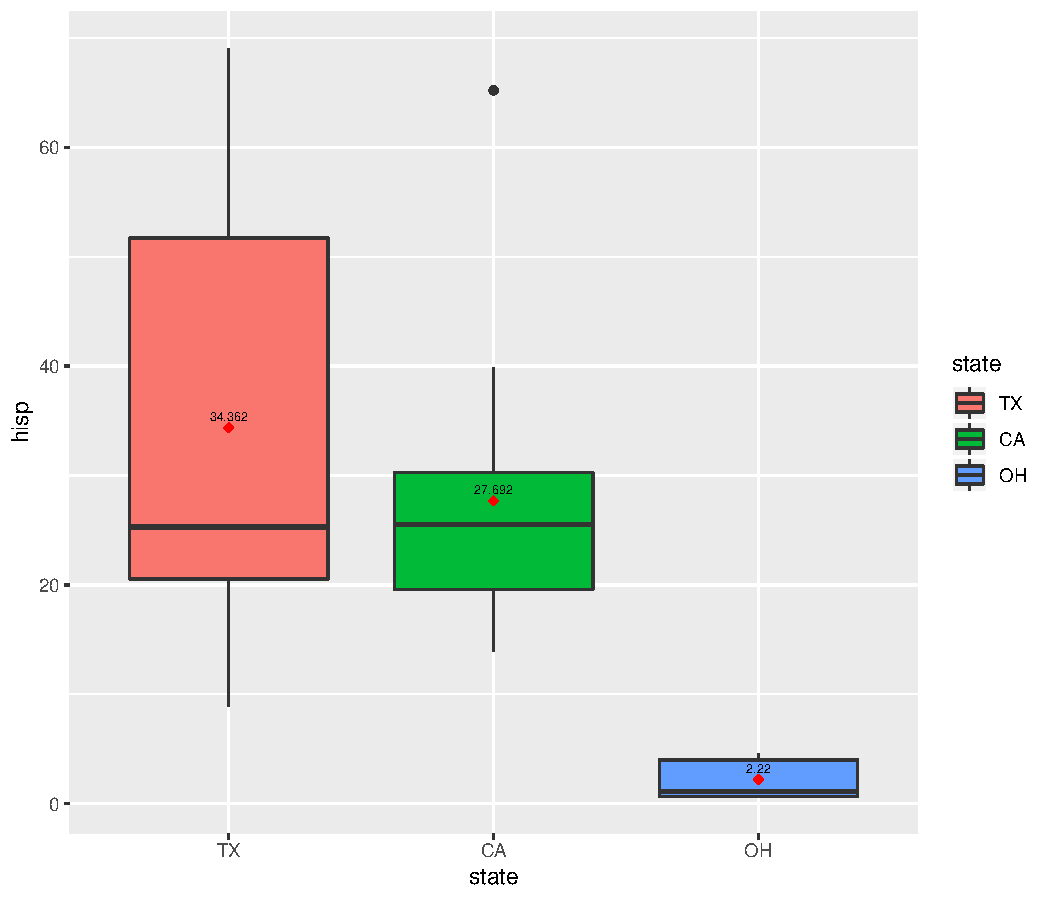
\includegraphics[width=\maxwidth]{figure/unnamed-chunk-18-1} 

\end{knitrout}


\end{document}
